\documentclass[10pt]{beamer}

%%%
% PREAMBLE FOR THIS DOC 
%%%
%https://tex.stackexchange.com/questions/68821/is-it-possible-to-create-a-latex-preamble-header
\usepackage{/Users/miw267/Repos/csci246_spring2025/slides/preambles/beamer_preamble_for_CSCI246}



%%% TRY TO RESHOW TOC AT EACH SECTION START (with current section highlighted)
% Reference: https://tex.stackexchange.com/questions/280436/how-to-highlight-a-specific-section-in-beamer-toc
\newcommand\tocforsect[2]{%
  \begingroup
  \edef\safesection{\thesection}
  \setcounter{section}{#1}
  \tableofcontents[#2,currentsection]
  \setcounter{section}{\safesection}
  \endgroup
}


%%%% HERES HOW TO DO IT CORRECTLY
% FIRST IN .STY FILE, DO
%\usetheme[sectionpage=none]{metropolis}
% THEN AT EACH SECTION DO
%\begin{frame}{Outline}
%  \tableofcontents[currentsection]	
%\end{frame}



%\setbeamertemplate{navigation symbols}{}
%\setbeamertemplate{footline}[frame number]{}


%%%
% DOCUMENT
%%%

\begin{document}

%\maketitle

%% Title page frame
%\begin{frame}
%    \titlepage 
%\end{frame}





\title{02/26/2025: Equivalence Relations}
\author{CSCI 246: Discrete Structures}
\date{Textbook reference: Sec 15, Scheinerman}

\begin{frame}
    \titlepage 
\end{frame}


\begin{frame}
\footnotesize 
\begin{mygreenbox}[title=Graded Quiz Pickup]
Quizzes are in the front of the room, grouped into four bins (A-G, H-L, M-R, S-Z) by last name. The quizzes are upside down with your last name on the back. Come find yours before, during, or after class.  Only turn the quiz over if it's yours.
\end{mygreenbox} 
\vfill 

\begin{myredbox}[title=Announcements]

This Friday's problem quiz will cover relations (including equivalence relations) - see slide decks from 2/19, 2/24, and 2/26.  \\

Next Friday's problem quiz will cover partitions and functions

\end{myredbox}

\vfill 


\begin{myyellowbox}[title=Today's Agenda]
\begin{itemize}
	\item Reading quiz (10 mins)
	\item Mini-lecture ($\approx$ 20 mins)
%	%
%	\begin{itemize}
%	\footnotesize 
%	\item Review induction 
%	\end{itemize}
%	%
	\item Group exercises ($\approx$ 15 mins)
\end{itemize}

%	Rationale for group exercises: we got shortchanged on time last couple days, and I already did a lot of lectures, so I want you to practice. Next problems quiz will cover relations and functions: Hamkins and 
%	
\end{myyellowbox}
\vfill 

\end{frame}

\begin{frame}
 \begin{myredbox}[title=Reading Quiz (Equivalence Relations) (Extra Credit)]  
 Prove the theorem below. 
\end{myredbox}
\vfill 
\begin{myyellowbox}[title=Theorem]
Let $n$ be a positive integer.  Congruence modulo $n$ is an equivalence relation on the set of integers.
\end{myyellowbox}
\vfill 
\begin{mygreenbox}[title=Definition]
Let $n$ be a positive integer.  We say that integers $x$ and $y$ are \textbf{congruent modulo n}, and we write 
\[x \equiv y \quad \text{(mod $n$)} \]
if $n | (x-y)$.
\end{mygreenbox}
\vfill 
%\textbf{Remark.} For intuition, note that $x \equiv y$ (mod $n$) if $x$ and $y$ have the same remainder after dividing by $n$.  For example, $6 \equiv 1$ (mod 5).
\end{frame}

\begin{frame}{Solution to reading quiz}
\small 
\pause 
We verify the three properties of an equivalence relationship below. 

\begin{itemize}
\item \textit{Reflexivity}: \pause  We need to check $xRx$. That is, we need to check $n|(x-x)$. In other words, we need to check $n|0$.  By definition of divisibility, we need to check that there is an integer $c$ such that $nc=0$.  This is satisfied by setting $c=0$. \; \greencheck 
\item \textit{Symmetry}:\pause   \; We need to check that if $xRy$ , then $yRx$.  In other words, we need to check that if $n|(x-y)$, then $n|(y-x)$.  Let $n|(x-y)$. Then there is an integer $c$ such that $nc = x-y$.  Hence $n(-c) = y-x$.  So $n|(y-x)$.  \; \greencheck  
\item \textit{Transitivity}:  \pause  We need to check that if $xRy$ and $yRz$ , then $xRz$.   That is, we need to check that if $n|(x-y)$ and $n|(y-z)$, then $n|(x-z)$.  By assumption, there are integers $c$ and $d$ such that $nc=(x-y)$ and $nd=(y-z)$.  Now we write
 	\[ x-z = (x-y) + (y-z) = nc + nd = n(c+d).\]
 	Since $c+d$ is an integer, clearly $n|x-z$. \; \greencheck
\end{itemize}
\end{frame}

\begin{frame}
\small 
 \begin{myredbox}[title=Remark (which may help with intuition)]  
For intuition, note that $x \equiv y$ (mod $n$) if and only if $x$ and $y$ have the same remainder after dividing by $n$.  For example, $4 \equiv 1$ (mod 3).	 
\end{myredbox}
\vfill 
\begin{mygreenbox}[title=Definition]
Let $R$ be an equivalence relation on a set $A$ and let $a \in A$.   The \textit{equivalence class} of $a$, denoted $[a]$, is the set of all elements of $A$ related (by $R$) to $a$.  That is,
\[  [a] = \set{x \in A: xRa}\]
\end{mygreenbox}
\vfill 
\begin{myyellowbox}[title=Example]
The integers can be partitioned into the following equivalence classes
%
\begin{align*}
[0] &= \set{\hdots, -6, -3, 0, 3, 6, \hdots} \\	
[1] &= \set{\hdots, -5, -2, 1, 4, 7, \hdots} \\	
[2] &= \set{\hdots, -4, -1, 2, 5, 8, \hdots} \\	
\end{align*}
%
under the relation of congruence mod 3.
\end{myyellowbox}

\end{frame}


\begin{frame}{Application: Public-Key Cryptography}
\footnotesize 
\begin{figure}[ht]
        \centering
        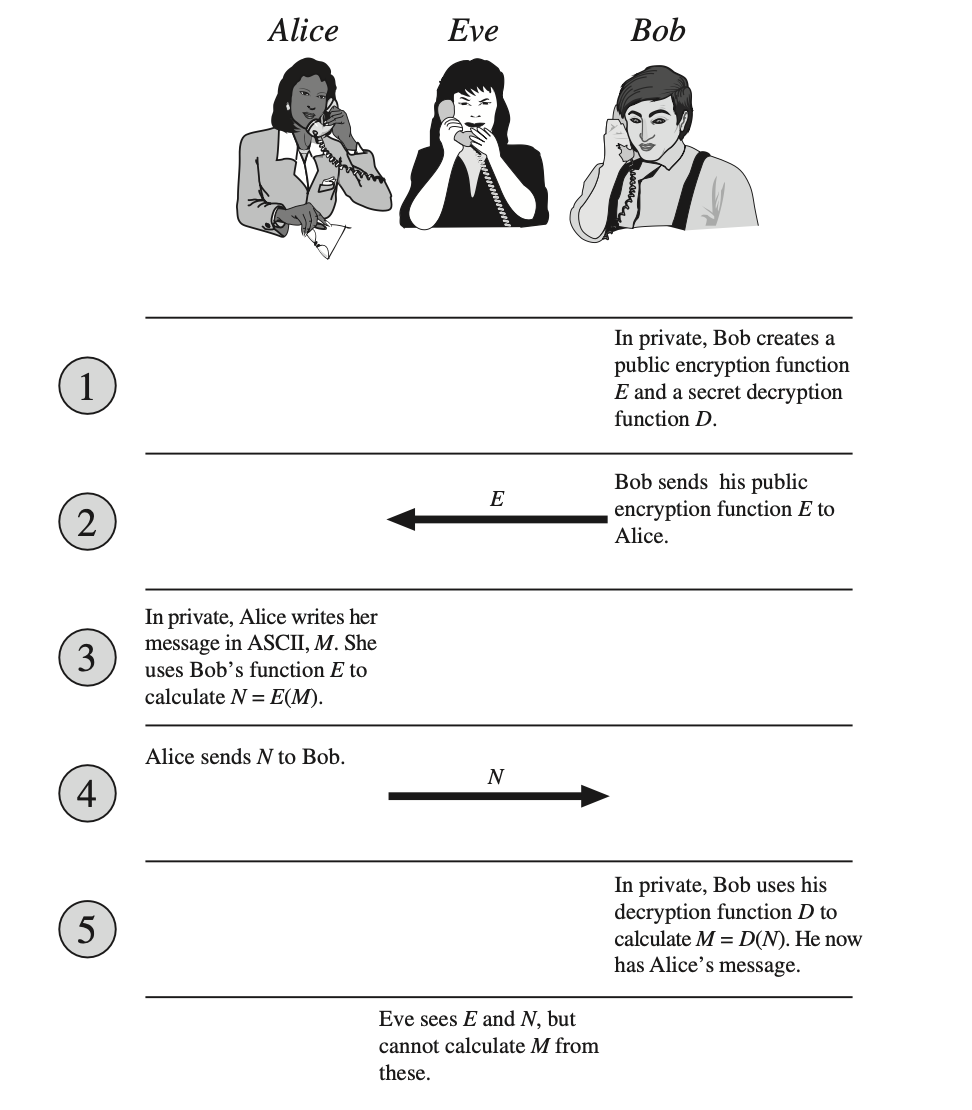
\includegraphics[width=.65\textwidth]{images/cryptography}
   		 %\caption{Median Score = 4/4 (100\%)}
\end{figure}
\vfill 
\end{frame}




\begin{frame}[standout]
Feedback on Monday's Quiz	
\end{frame}


\begin{frame}{Scores On Reading Quiz (Relations)}
\footnotesize 
\begin{figure}[ht]
        \centering
        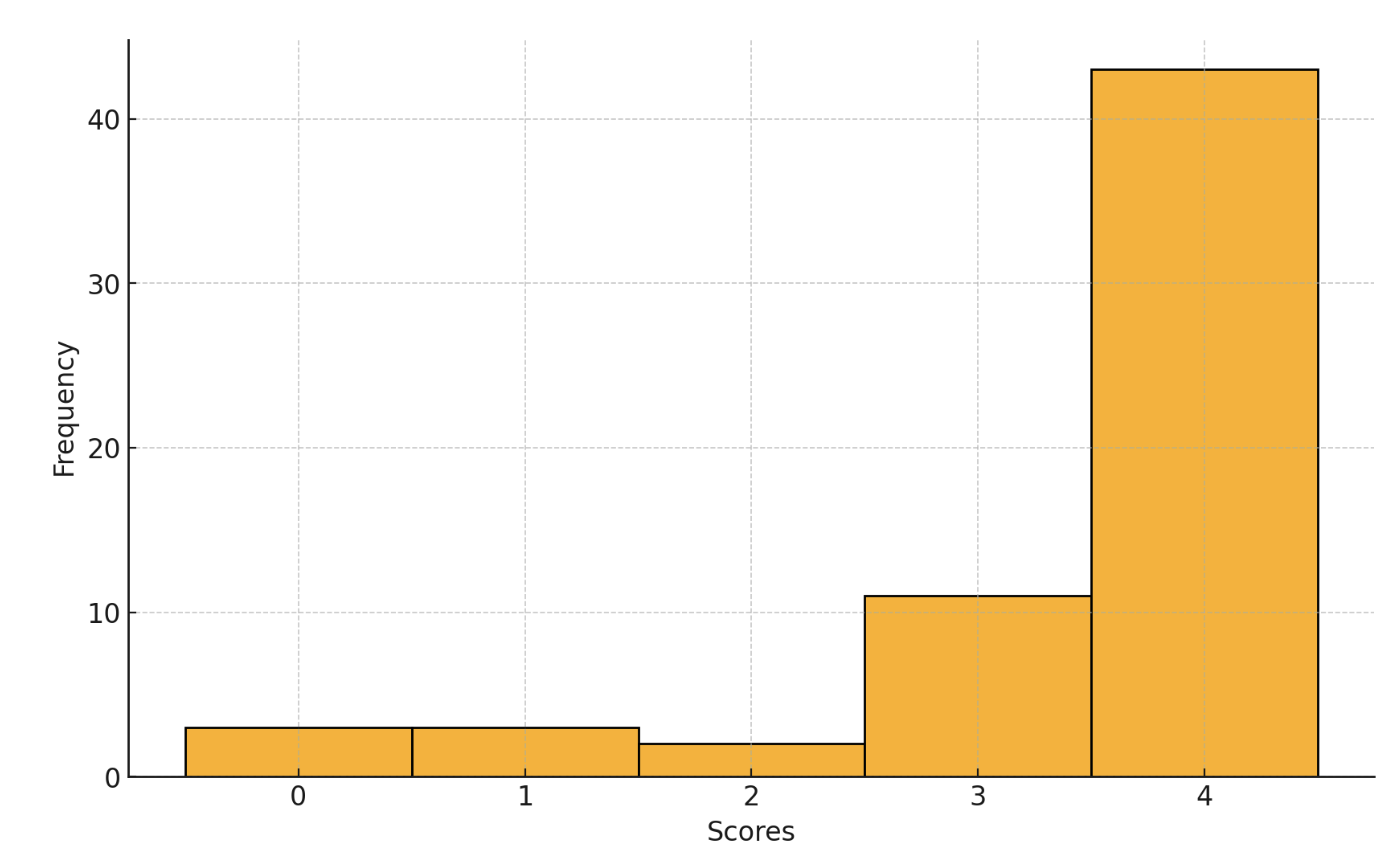
\includegraphics[width=.75\textwidth]{images/reading_quiz_scores}
   		 \caption{Median Score = 4/4 (100\%)}
\end{figure}
\vfill 
\textbf{Rubric.}  1 point for each subquestion if correct.

\end{frame}

\begin{frame}[standout]
Q\&A On Previous Group Exercises
\end{frame}

\begin{frame}[standout]
Group exercises
\end{frame}

\begin{frame}
\footnotesize 
\vfill 
\begin{columns}
\begin{column}{0.33\textwidth}
aaron.loomis: 11 \\ 
adam.wyszynski: 6 \\ 
alexander.goetz: 19 \\ 
alexander.knutson: 8 \\ 
anthony.mann: 14 \\ 
blake.leone: 10 \\ 
bridger.voss: 9 \\ 
caitlin.hermanson: 20 \\ 
cameron.wittrock: 16 \\ 
carsten.brooks: 15 \\ 
carver.wambold: 6 \\ 
colter.huber: 17 \\ 
conner.reed1: 22 \\ 
connor.graville: 7 \\ 
connor.mizner: 3 \\ 
connor.yetter: 1 \\ 
delaney.rubb: 8 \\ 
derek.price4: 19 \\ 
devon.maurer: 14 \\ 
emmeri.grooms: 13 \\ 
erik.moore3: 3 \\ 
ethan.johnson18: 4 \\\end{column}
\begin{column}{0.33\textwidth}
evan.barth: 18 \\ 
evan.schoening: 9 \\ 
griffin.short: 17 \\ 
jack.fry: 3 \\ 
jacob.ketola: 18 \\ 
jacob.ruiz1: 7 \\ 
jacob.shepherd1: 10 \\ 
jada.zorn: 22 \\ 
jakob.kominsky: 12 \\ 
james.brubaker: 22 \\ 
jeremiah.mackey: 5 \\ 
jett.girard: 21 \\ 
john.fotheringham: 2 \\ 
jonas.zeiler: 14 \\ 
joseph.mergenthaler: 11 \\ 
joseph.triem: 21 \\ 
julia.larsen: 10 \\ 
justice.mosso: 6 \\ 
kaden.price: 5 \\ 
lucas.jones6: 5 \\ 
luka.derry: 18 \\ 
luke.donaldson1: 2 \\\end{column}
\begin{column}{0.33\textwidth}
lynsey.read: 1 \\ 
mason.barnocky: 20 \\ 
matthew.nagel: 16 \\ 
micaylyn.parker: 2 \\ 
michael.oswald: 9 \\ 
nolan.scott1: 15 \\ 
owen.obrien: 13 \\ 
pendleton.johnston: 7 \\ 
peter.buckley1: 19 \\ 
peyton.trigg: 21 \\ 
reid.pickert: 11 \\ 
ryan.barrett2: 12 \\ 
samuel.hemmen: 16 \\ 
samuel.mosier: 1 \\ 
samuel.rollins: 15 \\ 
sarah.periolat: 17 \\ 
timothy.true: 20 \\ 
tristan.nogacki: 4 \\ 
tyler.broesel: 12 \\ 
william.elder1: 13 \\ 
yebin.wallace: 4 \\ 
zeke.baumann: 8 \\\end{column}
\end{columns}
\end{frame}



\begin{frame}{Group exercises}
\footnotesize 
\begin{enumerate}
	\item Which of the following are equivalence relations?
	\begin{itemize} \footnotesize 
	\item[a.] $|$ on $\mathbb{Z}$.
	\item[b.] $\leq$ on $\mathbb{Z}$.
	\item[c.] Is-an-angram-of on the set of English words. (For instance, \texttt{STOP} is an anagram of \texttt{POTS} because we can form one from the other by rearranging its letters.)
	\item[d.] $R=\set{(1,2),(2,3),(3,1)}$ on the set $\set{1,2,3}$.
	\item[e.] $\set{1,2,3} \times \set{1,2,3}$ on the set $\set{1,2,3}$.
	\item[f.] $\set{1,2,3} \times \set{1,2,3}$ on the set $\set{1,2,3,4}$.
	\end{itemize}
	\item For each equivalence relation below, find the requested equivalence class(es).
	\begin{itemize} \footnotesize 
	\item[a.] $R=\set{(1,1), (1,2), (2,1), (2,2), (3,3), (4,4)} $ on $\set{1,2,3,4}$. Find $[1],[2],[3],[4]$
	\item[b.] $R$ is has-the-same-tens-digit on the set $\set{x \in \mathbb{Z} : 100 < x < 200}$.  Find [123].
	\item[c.] $R$ is has-the-same-parents-as on the set of all human beings.  Find [you].
	\item[d.] $R$ is has-the-same-size-as on $2^{\set{1,2,3,4,5}}$.  Find $[\set{1,3}]$.
	\end{itemize}
\item Prove Proposition 15.11:  Let $R$ be an equivalence relation on the set $A$ and let $a,x,y \in A$. If $x,y \in [a]$, then $xRy$.
\end{enumerate}
	
\end{frame}


\begin{frame}{Solution to group exercise \#1}
\footnotesize 
\textbf{Problem.} Which of the following are equivalence relations?
	\begin{itemize} \footnotesize 
	\item[a.] $|$ on $\mathbb{Z}$.
	\item[b.] $\leq$ on $\mathbb{Z}$.
	\item[c.] Is-an-angram-of on the set of English words. (For instance, \texttt{STOP} is an anagram of \texttt{POTS} because we can form one from the other by rearranging its letters.)
	\item[d.] $R=\set{(1,2),(2,3),(3,1)}$ on the set $\set{1,2,3}$.
	\item[e.] $\set{1,2,3} \times \set{1,2,3}$ on the set $\set{1,2,3}$.
	\item[f.] $\set{1,2,3} \times \set{1,2,3}$ on the set $\set{1,2,3,4}$.
	\end{itemize}
	\vfill 
\textbf{Solution.}
	\begin{itemize} \footnotesize 
	\item[a.] No, because the relation is not symmetric.  For example, $3R6$ but $6\cancel{R}3$. 
	\item[b.] No, because the relation is not symmetric. For example, $3R4$ but $4\cancel{R}3$. 
	\item[c.] Yes. 
	\item[d.] No, because the relation is not transitive.  In particular, we have $1R2$ and $2R3$, but $1 \cancel{R} 3$.  %(The relation contains $(1,2)$ and $(2,3)$ but not $(1,3).$)
	\item[e.] Yes. 
	\item[f.] No, because the relation is not reflexive. In particular, $4 \cancel{R} 4$. 
	\end{itemize}
	
\end{frame}


\begin{frame}{Solution to group exercise \#2}
\footnotesize 
\textbf{Problem.} For each equivalence relation below, find the requested equivalence class(es).
	\begin{itemize} \footnotesize 
	\item[a.] $R=\set{(1,1), (1,2), (2,1), (2,2), (3,3), (4,4)} $ on $\set{1,2,3,4}$. Find $[1],[2],[3],[4]$
	\item[b.] $R$ is has-the-same-tens-digit on the set $\set{x \in \mathbb{Z} : 100 < x < 200}$.  Find [123].
	\item[c.] $R$ is has-the-same-parents-as on the set of all human beings.  Find [you].
	\item[d.] $R$ is has-the-same-size-as on $2^{\set{1,2,3,4,5}}$.  Find $[\set{1,3}]$.
	\end{itemize}
\vfill 
\textbf{Solution.} 
	\begin{itemize} \footnotesize 
	\item[a.] We have $[1]=[2]=\set{1,2}$, $[3]=\set{3}$, and $[4]=\set{4}$.
	\item[b.] We have $[123]=\set{120,121,122,123,124,125,126,127,128,129}$.
	\item[c.] The answer depends on who's answering.  I have one sister named Rachael, so for me, $[\text{me}]=\set{\text{me, Rachael}}$.
	\item[d.] We have 
	\[ [\set{1,3}] = \bigg\{ \set{1,2}, \set{1,3}, \set{1,4}, \set{1,5}, \set{2,3}, \set{2,4}, \set{2,5}, \set{3,4}, \set{3,5}, \set{4,5} \bigg\}.\]
	\end{itemize}
\end{frame}


\begin{frame}{Solution to group exercise \#3}
\textbf{Problem.}  Prove Proposition 15.11:  Let $R$ be an equivalence relation on the set $A$ and let $a,x,y \in A$. If $x,y \in [a]$, then $xRy$.
\vfill 
\textbf{Solution.}. By the definition of equivalence classes (Scheinerman Definition 15.6), we have
%
\[ [a] =\set{x \in A : xRa}.\]
%
Now by assumption, $x \in [a]$, so we have $xRa$.  Similarly, by assumption, $y \in [a]$, so we have $yRa$.  Since R is an equivalence relation, it is symmetric, and so $yRa \implies aRy$.   Now we have $xRa$ and $aRy$, so by transitivity (which holds since R is an equivalence relation), $xRy$.
\end{frame}

\end{document}
